\documentclass[tikz,border=2pt]{standalone}
\usepackage{tikz}
\usepackage{tikz}
\usepackage{lmodern}
\usetikzlibrary{calc,decorations.pathreplacing}

% Visual conventions follow the existing MRNC TikZ pictures: ordinary
% components use TikZ's normal 0.4pt stroke, with compact TeX labels.
\tikzset{
  nu fibre/.style={
    x=0.78cm,
    y=0.78cm,
    line width=0.4pt,
    line cap=round,
    line join=round
  },
  nu label/.style={
    font=\scriptsize,
    inner sep=1pt
  },
  nu annotation/.style={
    font=\scriptsize,
    inner sep=1pt
  },
  nu dots/.style={
    font=\small,
    inner sep=0pt
  }
}

\begin{document}

%I_0-II-t t=0 case

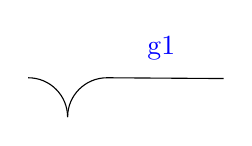
\begin{tikzpicture}[scale=0.5]
  \coordinate (A) at (-1.03, 6.95);
  \coordinate (B) at (0.11, 7.36);
  \coordinate (C) at (1, 8);
  \coordinate (D) at (3.96, 7.98);
  \coordinate (B_1) at (1.01, 7.00);
  \coordinate (E) at (2.38, 8.20);

  \draw (0, 7) arc (0.0:90.0:1.00);
  \draw (-0.9, 7.35) arc (180.0:180.0:1.00);
  \draw (1, 8.00) arc (90.0:180.0:1.00);
  \draw (C) -- (D);
  \node[above, text=blue] at (E) {g1
};
\end{tikzpicture}
\end{document}
